\chapter{Introduction}

Words are the building blocks of natural language. Words are categorized into word classes (for example verbs, nouns, adjectives) and any given grammar only allows certain combinations and word orders to form valid sentences. The meaning of these words is manifold, and naturally some words are more similar to each other than they are to others. Consider for example the three words ``interesting'', ``fascinating'' and ``bottle''. In this case, the first two words are more similar to each other.
Hence, the idea to represent words in a way that captures these similarities, is natural. One way of achieving this is the use of semantically informed vector representations, so-called word embeddings.

Finding suitable word embeddings is a challenging and interesting task. The objective is to find a low-dimensional vector for each word and/or phrase in the vocabulary. When done correctly, these word embeddings have been shown to be useful to help solving difficult Natural Language Processing (NLP) problems, including machine translation~\cite{Mikolov2013b, Wolf2013}, sentence completion~\cite{Mikolov2013a}, sentiment analysis~\cite{Hong}, and topic modeling~\cite{Jameel2013}.

Recent advancements~\cite{Mikolov2013a, Mikolov2013} allow finding high-quality low-dimensional word embeddings, while the processing speed is increased substantially due to many optimizations and/or approximations. Furthermore, reliable and fast implementations have been developed and released, one of them being Gensim~\cite{rehurek_lrec}. Therefore, training a word embedding model is now feasible within minutes or hours, while it took days or months before~\cite{Mikolov2013}.

For many applications, the data is formatted in a hierarchical structure, as can be observed in Figures~\ref{fig:1:hierarchies-wikipedia-syntax},~\ref{fig:1:hierarchies-categories} and~\ref{fig:1:hierarchies-sports}. Therefore, it is compelling to try exploiting these hierarchies to improve the quality of the word embeddings and/or to reduce the learning time while maintaining the word vector quality. To our best knowledge, this concept has not been investigated profoundly yet, using the recent advancements in~\cite{Mikolov2013}, although there have been motions towards this direction already~\cite{Fu2014}.

%todo tbd carsten: maybe include one more paragraph on why we think this should help and what it should achieve.

\begin{figure}
	\centering
	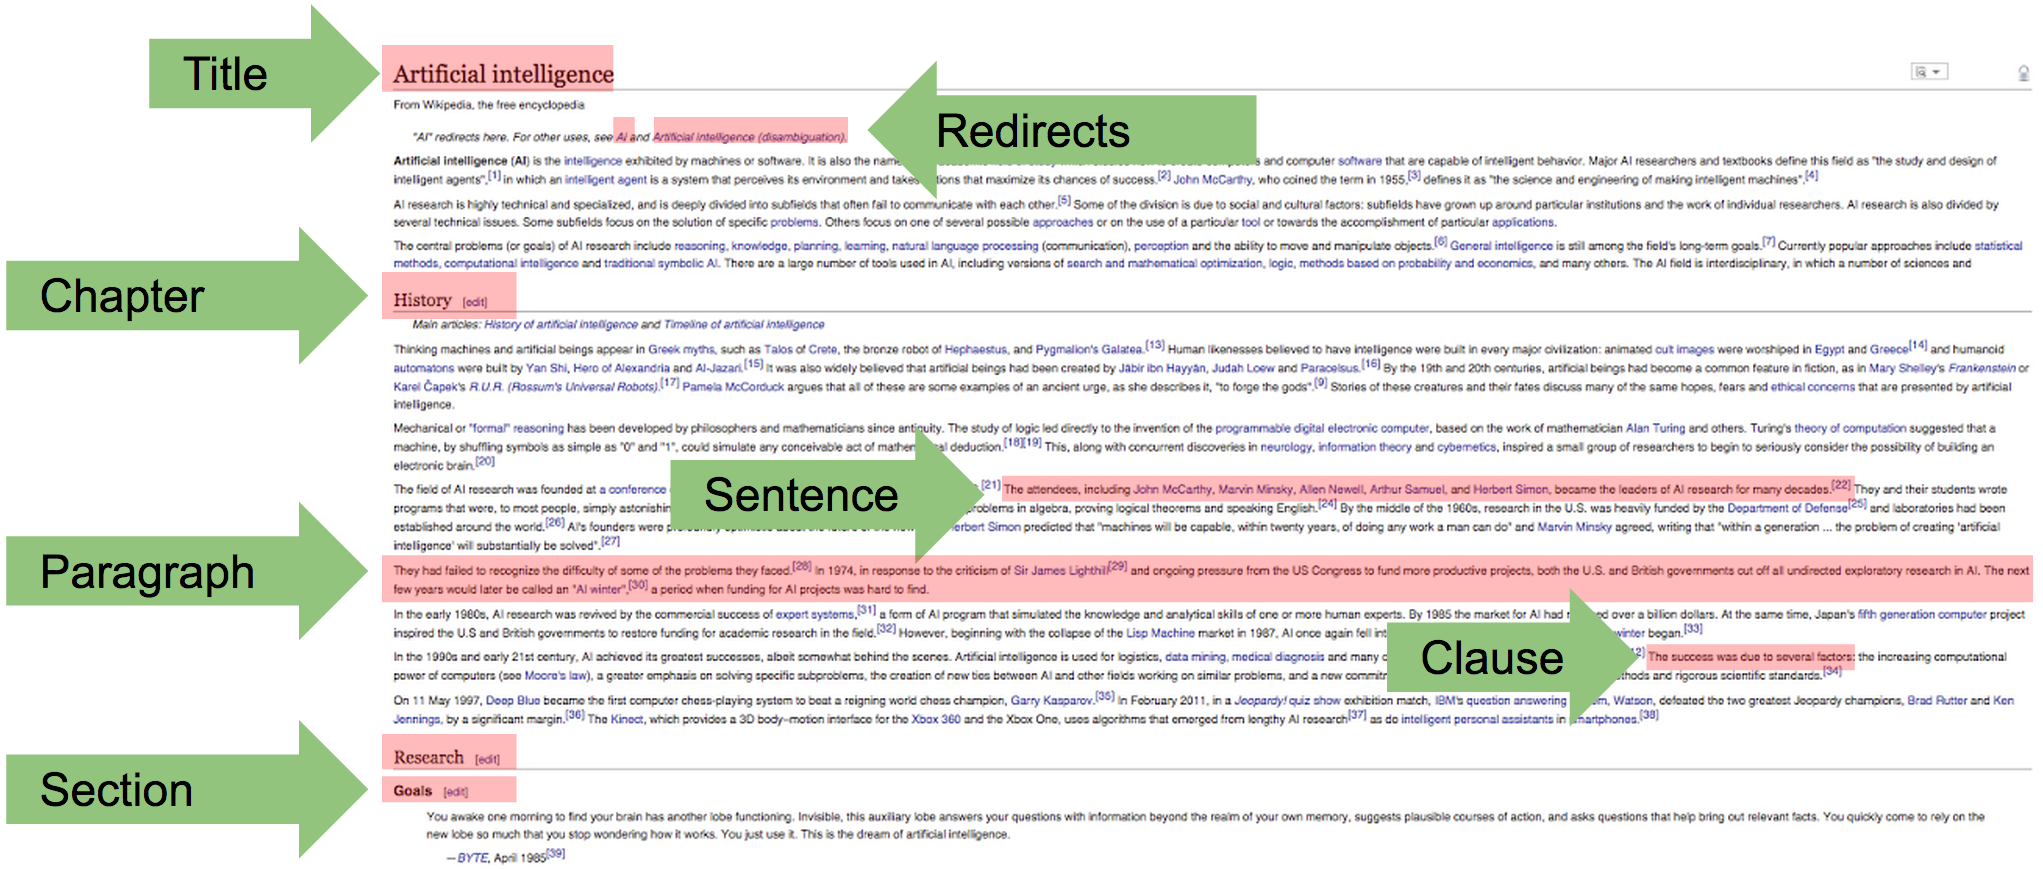
\includegraphics[width=1.0\textwidth]{1introduction/hierarchies-wikipedia-syntax.png}
	\caption[Caption for LOF]{The Wikipedia article about artificial intelligence is segmented into semantic and syntactic hierarchies (for example title, chapter, section, paragraph, sentence, clause).\footnotemark}
	\label{fig:1:hierarchies-wikipedia-syntax}
\end{figure}

\footnotetext{Source: \url{https://en.wikipedia.org/wiki/Artificial_intelligence}}

\begin{figure}
	\centering
	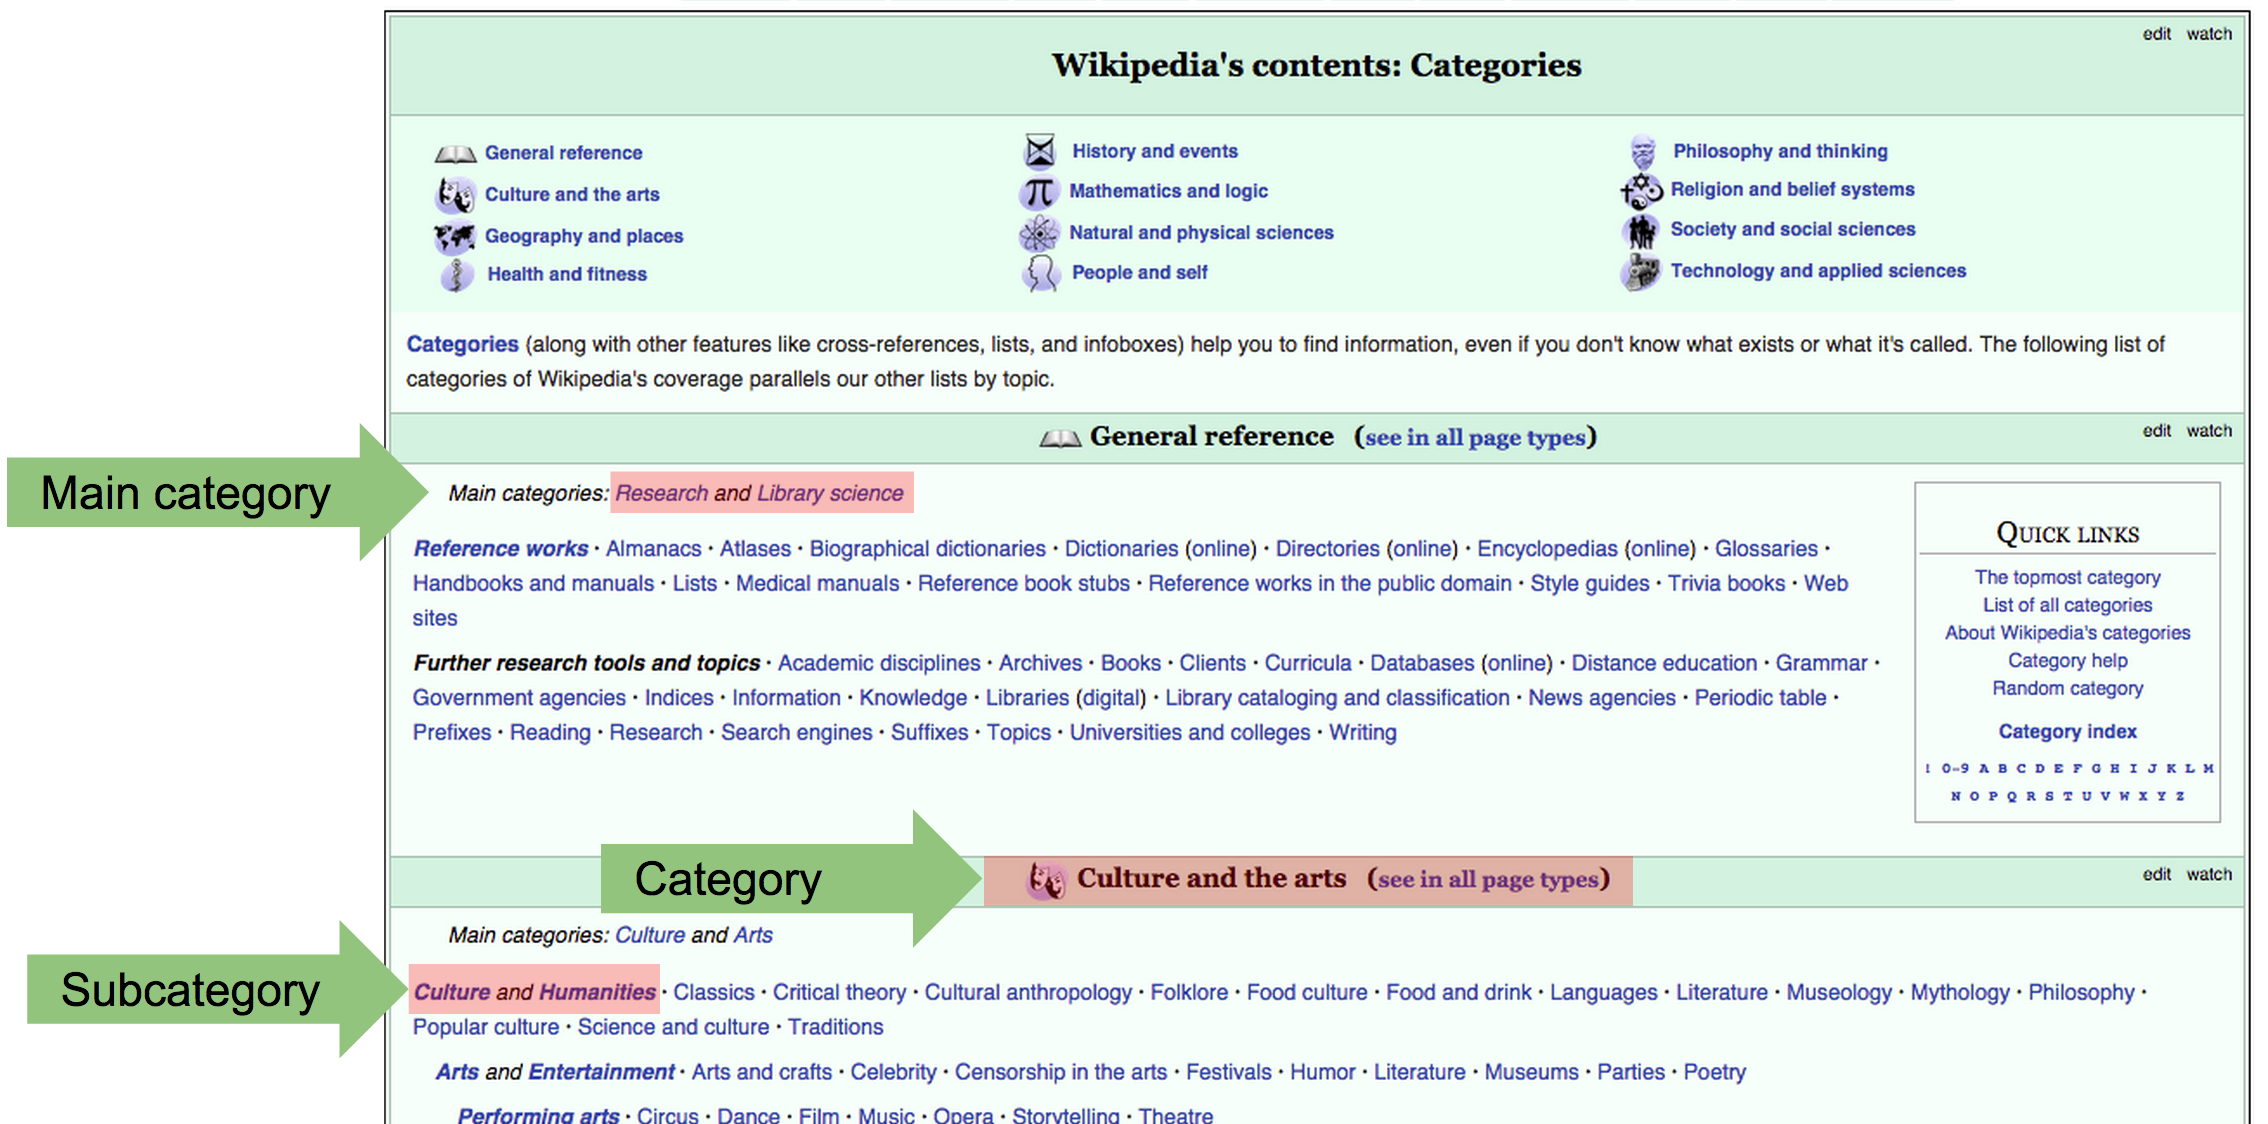
\includegraphics[width=1.0\textwidth]{1introduction/hierarchies-wikipedia-categories.png}
	\caption[Caption for LOF]{Wikipedia articles are structured in categories. For example, the article ``Bayes' theorem'' can be found in the hierarchy ``Bayesian statistics'' $<$ ``Statistics'' $<$ ``Mathematics and logic''.\footnotemark}
	\label{fig:1:hierarchies-categories}
\end{figure}

\footnotetext{Source: \url{https://en.wikipedia.org/wiki/Portal:Contents/Categories}}

\begin{figure}
	\centering
	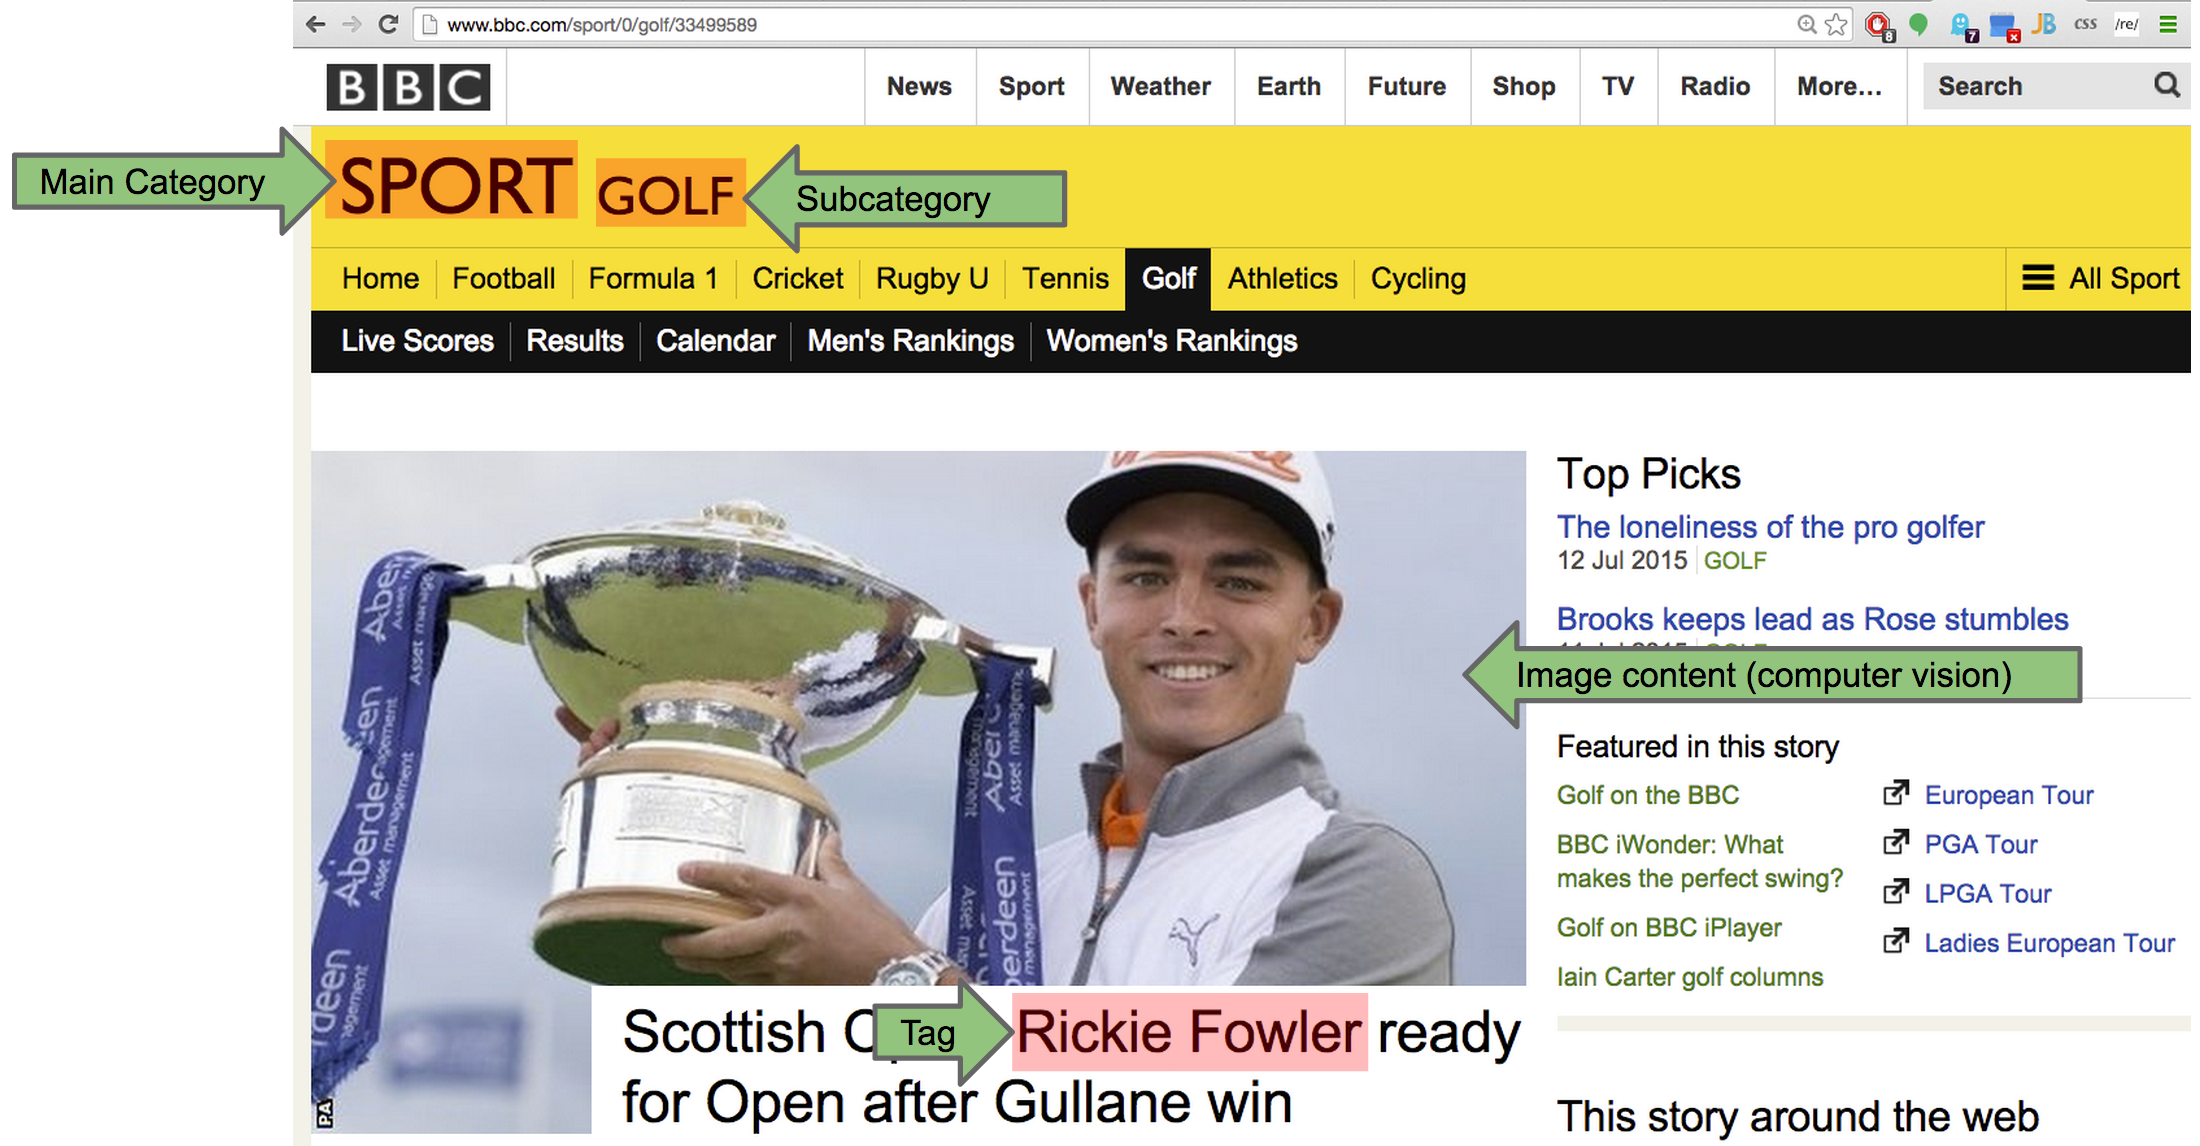
\includegraphics[width=1.0\textwidth]{1introduction/hierarchies-sports.png}
	\caption[Caption for LOF]{This sports article is categorized into the category ``sport'' and subcategory ``golf''. Additional tags (for example the name of the person who is on the picture) may also be available.\footnotemark}
	\label{fig:1:hierarchies-sports}
\end{figure}

This thesis is organized as follows: in Chapter~\ref{related-work}, related work underlying this thesis is discussed. Chapter~\ref{preliminaries} introduces theory needed to understand this thesis. Chapter~\ref{hierarchical-paragraph-vectors} investigates the formal core of this thesis by describing Hierarchical Paragraph Vectors. Chapter~\ref{experiments} describes the conducted experiments, and Chapter~\ref{conclusion-and-future-work} concludes the results and previews future work.

\newpage

\footnotetext{Source: \url{http://www.bbc.com/sport/0/golf/33499589}}
